% Chapter Template

\chapter{Evaluation}\label{ch:evaluation}


\section{Confis Project Goals}\label{sec:eval:goals}

This project hopes to leverage software engineering techniques (like domain-specific languages), existing logic abstractions (like normative rules), and existing technologies relating to law (like Ricardian contracts) in order to provide a framework allowing people with non-technical and non-legal backgrounds to draft, review, and access information in legal agreements.

The following criteria are motivated by how existing technologies in the state-of-the-art (see sections~\ref{sec:nlp} and~\ref{sec:machine-readable-contracts}) fail to address them:

\begin{definition}[Meaningful Representation]
    \label{def:meaningful-representation}
    Confis should be able to fully represent a legal agreement in a legal context.

    That is, (albeit with the use of tooling) a Confis agreement should be usable in place of a legal one.

\end{definition}

\begin{definition}[Accessibility]
    \label{def:accessibility}
    Whatever the encoding of a Confis agreement, should be possible to produce (albeit with the use of tooling) such Confis agreement without an in-depth understanding of the formalism that encodes the agreement.
\end{definition}

The following are loosely defined -- this is unavoidable because this project aims to introduce a formalisation for legal documents, which are not well-defined.
Please see~\nameref{sec:language-semantics} for the definitions of~\nameref{def:action},~\nameref{def:party},~\nameref{def:permission}, and~\nameref{def:requirement}.

% TODO revisit after writing reasoning section
\begin{definition}[Completeness]
    \label{def:completeness}
    A Confis agreement $C$ is complete with respect to a legal agreement $L$ if it represents $L$ and:

    \begin{itemize}
        \item If $L$ allows a legal capability $c$, then $C$ also allows $c$ through an equivalent permission
        \item If $L$ forbids a legal capability $c$, then $C$ also forbids $c$ through an equivalent permission
        \item If $L$ has a requirement $r$, then $C$ has $r$
    \end{itemize}
\end{definition}


\begin{definition}[Soundness]
    \label{def:soundness}
    A Confis agreement $C$ is sound with respect to a legal agreement $L$ if it represents $L$ and:

    \begin{itemize}
        \item If $C$ has an \texttt{Allow} permission $p$ equivalent to a capability $c$, then a $L$ also allows $c$
        \item If $C$ has a \texttt{Forbid} permission $p$ equivalent to a capability $c$, then a $L$ also forbids $c$
        \item If $C$ has a requirement $r$, then $L$ has $r$
    \end{itemize}
\end{definition}


\section{Language Formalism Evaluation}\label{sec:language-formalism-evaluation}

The Confis language formalism and semantics are discussed in~\autoref{sec:language-semantics}.
This project will evaluate it in how it meets the requirements described in~\autoref{sec:eval:goals}, its expressiveness (how capable it is to represent complex contracts) as well as how it performs in relation to comparable formalisms (like~\nameref{subsubsec:symboleo}~\cite{symboleo2020} or~\nameref{subsec:accord}~\cite{accordHomepage}).
Due to the nature of legal agreements (and the impossibility of formalising large amounts of existing legal contracts) this assessment is a qualitative one.

As far as fulfilling the~\nameref{def:accessibility} requirement, Confis is one of the few formalisms in the literature that makes an effort to penetrate industry by
\begin{itemize}
    \item Making few assumptions about the user's background (including knowledge such as event fluidity, event calculus, or first order predicate logic).
    \item Choosing language constructs to purposefully resemble natural language.
    \item Providing additional tools to ease development and shorten the iteration loop.
\end{itemize}

The Query UI~(\autoref{sec:queryUI}), Confis-to-English conversion~(\autoref{sec:additional-tooling:doc-rendering}), the Confis Editor~(\autoref{sec:confis-editor}) and the structure of the Confis language itself (\autoref{sec:language-semantics}) were all developed with this goal in mind.

Exceptions to this statement include accessible technologies like Juro (\autoref{subsec:juro}).
Such tools add contract metadata without actually allowing for querying beyond fetching the metadata, nor attempt to capture the semantics of the agreement -- like Adobe Signing tools or typical Ricardian Contracts~\cite{ricardianWeb}, but unlike Symboleo or The Accord Project.

We translate to Confis a sample contract used in Symbolio~\cite{symboleo2020} in order to compare the same agreement in two different languages.
For the sake of brevity, we wille examine an extract, but the full original (in plain English) can be found at~\autoref{tab:meat}, the full Symbolio specification at~\autoref{fig:symbolio:meatSales}, and the full Confis agreement at~\autoref{fig:confis:meat}.

\begin{table}[h]
    \centering
    \setlength{\fboxsep}{10pt}
    \fbox{
        \begin{minipage}{0.8\textwidth}
            \textbf{Confidentiality}
            \begin{enumerate}
                \item Both Seller and Buyer must keep the contents of this contract confidential during the execution of the contract and six months after the termination of the contract.
            \end{enumerate}
        \end{minipage}
    }
    \caption[Sample confidentiality clause]{Sample confidentiality clause, extracted from~\autoref{tab:meat}}
    \label{tab:meat-confidentiality}
\end{table}

The comparison will be performed on a rather simple clause of the agreement, a confidentiality clause specified by~\autoref{tab:meat-confidentiality}.
The Confis representation is specified by~\autoref{fig:confis:meat-confidentiality}, while the Symbolio one is specified by~\autoref{fig:symbolio:meatSales-confidentiality}.
Both are re-written self-contained examples (rather than text extracts from the original, longer contracts).
This was done in order to fully reflect the necessary boilerplate and ceremony of each language.


\begin{figure}[h]
    \centering
    \begin{minted}[
        autogobble,
        frame=lines,
        framesep=2mm,
        fontsize=\footnotesize
    ]{kotlin}
val effDate = 1 of June year 2022
val reveal by action(
    description = "as in not keeping the contents confidential"
)
val contract by thing("the Contract", description = "this Agreement")
val seller by party("the Seller", description = "Alice Liddell")
val buyer by party("the Buyer", description = "The Meat Supermarket, Inc")

seller mayNot reveal(contract) asLongAs {
    within { effDate..(effDate + 6.months) }
}

buyer mayNot reveal(contract) asLongAs {
    within { effDate..(effDate + 6.months) }
}
    \end{minted}
    \caption{Confis for~\nameref{tab:meat-confidentiality}, extracted from~\autoref{fig:confis:meat}}
    \label{fig:confis:meat-confidentiality}
\end{figure}

\begin{figure}[h]
    \begin{minted}[
        autogobble,
        frame=lines,
        framesep=2mm,
        fontsize=\footnotesize
    ]{prolog}
        Domain meatSaleDomain
        Seller isA Role with returnAddress: String, name: String;
        Buyer isA Role with warehouse: String;
        Disclosed isAn Event;

        endDomain

        Contract MeatSale (buyer: Buyer, seller: Seller, effDate: Date)

        Declarations
        disclosed: Disclosed;

        Surviving Obligations
        so1 : Obligation(seller, buyer, true,
            not WhappensBefore(disclosed, Date.add(Activated(self), 6, months))
        );

        so2 : Obligation(buyer, seller, true,
            not WhappensBefore(disclosed, Date.add(Activated(self), 6, months))
        );
        endContract
    \end{minted}
    \caption{Symboleo Specification for~\nameref{tab:meat-confidentiality}, extracted from~\autoref{fig:symbolio:meatSales}}
    \label{fig:symbolio:meatSales-confidentiality}
\end{figure}

\paragraph{Specifying a legal Obligation}
Notice how Symboleo allows representing a more complex domain by specifying an \emph{Event} \texttt{`Disclosed'}, and constraining the legal capabilities of Buyer by creating an \emph{Obligation} (with a notion of this obligation being \emph{from} Buyer \emph{towards} Seller) which specifies that the \texttt{disclosed} event cannot happen before six months after the end of the contract.
In Symbolio's model if \texttt{disclosed} happen, the breach cannot be attributed to either Seller nor Buyer.

Confis specifies a simpler domain -- while it also specifies Seller and Buyer and represents `disclosing' as an Action, it has no notion of \emph{creditor} and \emph{lender} when it comes to Requirements (defined in Definition~\autoref{def:requirement}).
On the other hand, Confis can `blame' specific parties for a breach, as it attributes Actions to Subjects.
Confis is also unable to keep track of its own execution time -- instead it requires specifying the date in the contract.
Notice how this abstracts away the document from the real-world execution date, and how this limitation of Symboleo is omitted in the original paper~\cite{symboleo2020}, but present in the sample source code~\cite{symboleoMeat}.

Both models are capable of expressing periods of time, but in Confis they are not part of the algebra (they are instead more general~\nameref{def:circumstance}s).

\paragraph{Accessibility}

While both contracts require language knowledge to write them, Confis can be read without prior training and its functions (\texttt{within}, \texttt{mayNot}, \texttt{asLongAs},~\dots) are easy to memorise.
The best example of this is the operation of summing six months to a time period -- while Symboleo requires specifying a \texttt{Date} library and wrapping the duration with a function (\texttt{`Date.add(..., 6, months)'}), Confis uses operator overloading to sum to a date (\texttt{`... + 6.months'}).

As far as readability goes, Confis goes the extra mile by trying to combine metadata and language semantics to provide an English-like preview.
This prose rendering is shown in~\autoref{fig:confis-render-meat-confidentiality}.
While the preview is not as clear as the original plain-English clause, it conveys the obligations of each party well and is unambiguous thanks to its definition referencing (which is common in real legal agreements).

\begin{figure}[H]
    \centering
    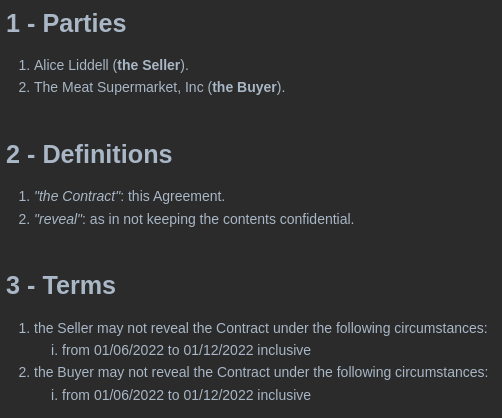
\includegraphics[width=0.67\columnwidth]{figures/confis.meat.prose}
    \caption{Confis prose rendering of~\autoref{tab:meat-confidentiality}}
    \label{fig:confis-render-meat-confidentiality}
\end{figure}

For a more detailed comparison of the specifications of this agreement in the Confis and Symboleo languages, please refer tor\autoref{ch:confis-examples}, in partcular~\autoref{subsec:meat-contract-comparison}.

\subsection{Confis Limitations in its Semantics}\label{subsec:confis-lang-limits}

While the focus Confis makes in Accessibility makes it easier to learn, read, and write;
it comes at a price in the guarantees it brings and the expressiveness of the contracts that it can represent.
% TODO solutions in future work?
This section provides a couple examples of clauses in existing contracts that Confis struggles to formalise and tries to generalise the situations it cannot encode, as well as suggesting solutions for the problem.

\subsubsection{Act Upon Violation}
\label{subsubsec:limits-violations}

Contracts are sometimes defensively written (not unlike defensive programming software engineering practices) where they may include clauses that specify what should happen upon breach of other clauses (an example of such a clause is given in~\autoref{tab:meat-breach}).

\begin{table}[h]
    \centering
    \setlength{\fboxsep}{10pt}
    \fbox{
        \begin{minipage}{0.9\textwidth}
            \textbf{Payment \& Delivery}
            \begin{itemize}
                \item In the event of late payment of the amount owed due, the Buyer shall pay interests equal to <intRate> the Seller may suspend performance of all of its obligations under the agreement until payment of amounts due has been received in full.
            \end{itemize}
        \end{minipage}
    }
    \caption[Sample breach clause]{Sample breach clause, extracted from~\autoref{tab:meat}}
    \label{tab:meat-breach}
\end{table}

In Confis semantics, this represents a contradiction in the logic of the contract, because we have a rule specifying that a set of states is a breach, and then other rules specifying capabilities when in those states.
This compromise between contradiction detection (extremely useful for helping the drafter produce well-formed contracts) and expressiveness (allowing these do-in-case-of-breach clauses) is unavoidable in the current semantics of Confis Allowance~(see~\nameref{def:allowance} for more details).

In order to circumvent this limitation, it is possible to create two `cases': a Permission that allows paying on time, and different Permission that allows paying at any time with interest.
While this removes the contradiction, it does not capture the violation semantics of the original legal agreement.

Symboleo is capable of capturing such a scenario thanks to its \texttt{Happens(Violated(\_))} predicate, which can create a new obligation when a different obligation is violated.

\subsubsection{Confis Does Not Have Time in its Event Algebra}
\label{subsubsec:limits-time}

Symboleo (and other logic-based solutions like~\cite{knottenbeltContractDriven}) relate events through \emph{happensBefore} partial orderings (introduced by~\cite{kowalski1989logicEventBased}).
They then can use these relations to model enforcing conditions, pre-conditions, and post-conditions over periods of time.

Confis only has a concept of time as a~\nameref{def:circumstance} -- an event does not necessarily happen at a given time, the same way it does not necessarily happen with a given purpose.
Ordering of events is established with an additional circumstance called a Past Action.
Again, this Circumstance does not receive special treatment and like the others it is up to the author of the contract to specify it.

While this design choice greatly simplifies rule generation and language semantics (thus making Confis easier to learn) it is a sacrifice in expressiveness.

For example, unlike Symboleo, Confis is unable to allow a new Capability only after an event $E$ occurred at a time $t$ and $E$ has happened after another event $E_{\text{past}}$.
Instead, Confis only allows a new capability after $E$ and $E_{\text{past}}$ have both happened, regardless of whether $E$ happened at time $t$, or whether $E$ happened before or after $E_{\text{past}}$.

It is possible to mitigate this issue by explicitly forbidding $E_{\text{past}}$ to happen before $E$ -- but then we would be slightly altering the original contract's semantics by introducing a new clause breach scenario.

\subsubsection{Confis Does Not Model Amounts}
\label{subsubsec:limits-amounts}

A key barrier to accessibility in existing formalisms -- and even any general-purpose programming language -- is their type systems.
Other than the absolutely necessary abstractions for the domain (such as Parties or Actions) users need to know what a strictly positive integer or a floating point number are.
The language then usually needs to define operations on these types, as well as extend them with other types such as Dates, Lists, etc.

Confis lowers the entry barrier by doing without most of this mental overhead (the only type concerned with numerical values it allows is a Date).
It does not require using libraries in order to perform operations -- mostly because there are no such operations, but partly thanks to operator overloading like in \autoref{fig:confis:meat-confidentiality}.

This greatly limits its expressiveness in terms of numerical amounts and the computations that can be done on them during the contract evaluation.
Consider The Accord Project~\cite{accordHomepage}~(see~\autoref{subsec:accord}), which models programs computationally with a more general-purpose language.
It is able to perform complex floating-point arithmetic in order to compute interest rates and fees, such as the one given in~\autoref{tab:economist-interest}.

On the other hand, Symboleo (and similar logic-based technologies) struggle more to perform such time-based calculations (possibly due to their declarative nature).
In the original Symboleo paper~\cite{symboleo2020} which contains a meat sales example hand-picked to showcase the language, the authors do not attempt to perform an interest calculation over time even though their original agreement (given in~\autoref{tab:meat}) specifies one -- this is shown in~\autoref{fig:symbolio:meat-interest} for convenience.

\begin{figure}[h]
    \centering
    \begin{minipage}{0.85\textwidth}
        \begin{minted}[
            autogobble,
            frame=lines,
            framesep=2mm,
            fontsize=\small
        ]{prolog}
        Domain
        Currency isAn Enumeration(CAD, USD, EUR);
        PaidLate isAn Event with
            amount: Number, currency: Currency, from: Buyer, to: Seller;

        Contract MeatSale (
            buyer : Buyer,
            seller : Seller,
            curr : Currency,
            interestRate: Number
        )

        endDomain

        Declarations
        paidLate: PaidLate with
            % where interestRate is a constant
            amount := (1 + interestRate / Math.abs(2)),
            currency := curr,
            from := buyer,
            to := seller;
        \end{minted}
    \end{minipage}
    \caption{Symboleo extract from~\autoref{fig:symbolio:meatSales} concerned with interest rates}
    \label{fig:symbolio:meat-interest}
\end{figure}

In short, while Confis lacks the computational capabilities of a programming language, it is not lacking when compared to Symboleo since it does allow specifying numerical constants (except without having to specify their types).
Additionally, traditional contracts also tend to leave to the reader such computations.

\begin{table}[h]
    \centering
    \setlength{\fboxsep}{10pt}
    \fbox{
        \begin{minipage}{0.9\textwidth}
            \textbf{Payment Terms}
            \begin{itemize}
                \item
                \ [\dots]
                Payments made after the due date may be [\dots] subject to a late fee equal to the lesser of 1.5\% per month or the maximum allowed by law.
            \end{itemize}
        \end{minipage}
    }
    \caption[The Econoimist licence interest rate clause]{Clause concerning an interest rate, extracted from~\cite{economistIU2016licence}, a Licence Agreement by The Economist Group}
    \label{tab:economist-interest}
\end{table}

\subsubsection{Confis Circumstances Are Domain-Aware}
\label{subsubsec:limits-domain-circumstances}

A Circumstance is an instance of an object that implements the functions given in Definition~\autoref{def:circumstance}.
These operations vary greatly depending on the domain that the Circumstance is meant to represent.
For example, for time-type Circumstances, the \texttt{overlapsWith} function checks for overlaps in time ranges;
while in past-event-type Circumstances \texttt{overlapsWith} checks the union of the sets of past events.
This makes Circumstances very intuitive to use in practice: if the contract specifies Alice must pay this week and she paid this Monday, she expects `Monday' to be generalised by `this week', without needing to learn about the abstractions behind Circumstances.


The price to be paid for this ease-of-use is that Circumstances for new domains must be implemented before they can be used.
The most simple example is geographical locations.
This Circumstance is not already built into Confis.
If we were to make such an extension to the language, we would need to define a location-type circumstance as some coordinates (or perhaps an address).
The functions \texttt{generalises} and \texttt{overlapsWith} would compare coordinates in order to determine if one is a location included in the other (say, a house within a street), or if they are close enough to be the same place.

In short, making domains accessible at the language level requires less general abstractions that require domain knowledge at the implementation level.
While Confis is built to be easily extensible implementation-wise, this is a rare limitation in specification languages, which usually aim to be as general as possible in order to cover all possible cases.
The trade-off is once again in accessibility and expressiveness, and can be circumvented by encoding a Circumstance inside a~\nameref{def:sentence}'s~\nameref{def:action} -- following the previous example, rather than `deliver', the Action can be rewritten as `deliver to 10 Downing St.'.

\subsection{Gravity of Language Semantics Limitations}\label{subsec:gravity--lang-limits}

This subsection aims to determine to what extent the limitations presented in~\autoref{subsec:confis-lang-limits} affect negatively the practical usability of Confis.
Given how Confis is superior in its accessibility to comparable languages in the literature like Symboleo and The Accord Project (by virtue of the compromises it makes) we have focused on comparing real-world contracts with their Confis representations, including~\cite{economistIU2016licence, symboleoMeat, jetbrainsToolbox, seismicDataLicence}.

The main discrepancies between the intended meaning of the plaintext agreements and their Confis counterparts concern re-evaluation of legal capabilities and obligations (ie, Confis'~\nameref{def:permission} and~\nameref{def:requirement}) when the state-of-the-world changes.
This includes the~\nameref{subsubsec:limits-violations} and~\nameref{subsubsec:limits-time} limitations.
Other lacks in expressiveness (like~\nameref{subsubsec:limits-domain-circumstances}) can be more easily circumvented by adapting Sentences to convey the intended meaning and by splitting clauses into several such Sentences.

Full examples of such discrepancies can be found in the code archive, as well as in~\autoref{ch:confis-examples}.

% TODO and is this ok??

\section{Software Deliverables}\label{sec:software-deliverables}

\subsection{Language Implementation}

\begin{itemize}
    \item \textbf{Coverage} 92.8\%
\end{itemize}

\subsection{Querying Engine}

\begin{itemize}
    \item \textbf{Coverage} 81.6\%
\end{itemize}

\subsection{Tooling Implementation: Legal Prose Rendering}

\begin{itemize}
    \item \textbf{Coverage} 94.6\%
\end{itemize}

\subsection{Tooling Implementation: Editor and Query UI}


\section[Overall Evaluation]{Overall Evaluation With Respect to Goals}


\section{Machine Readable Licence Representations}\label{sec:licence-representations}

% we are looking to eavaluate the project - a lot of this should go into the intro probably...

% measures will be cost (smart contracts!), lawyer avoidance, and advice from people that know about this stuff

Other goals of this project require that a legal agreement can be encoded for it to become
structured data.
The project should come up with, or find in the literature and adapt, a suitable format for a legal
agreement.
In order to limit the scope of the project, we will narrow the agreement to be encoded to
licences.

A successful project should include:
\begin{itemize}
    \item \textbf{Machine-readable representation of licenses}.
    \item \textbf{Prototype Software} that uses the contract representation to ease the existing
    manual workflow related to agreements in a business.
    This could include a searchable database that is aware of licenses related to the same data or
    software~(see~\ref{sec:contract-registry}).
    The software should, to some extent, allow querying a contract to be able to determine the
    conditions which the license allows to use the data in.
    \item Secure, \textbf{self-executing clauses} that all parties bound to the contract can trust.
    This includes making it so parties cannot have plausible deniability or repudiation if they are
    dishonest.
\end{itemize}

Legal contracts are complex documents that may list vague or hard-to-encode conditions and
situations.
I expect not being able to (inexpensively) capture the entire meaning of a contract in a
machine-readable format.
This disassociation between reality and representation should be fully taken into account when
providing guarantees and making assumptions.
For example, a successful prototype should be aware of this enough to refer the user to the original
license when it is unable to provide certainties with respect to a query against a license.

In other words, this uncertainty created by attempting to represent a contract in a machine-readable
encoding should be part of the encoding itself, for the sake of completeness and usability.

Evaluation criteria would include whether the project can successfully encode a wide range of
licence agreements.


\section{A Universal Contract Registry}\label{sec:contract-registry}

A decentralised contract registry, shared by multiple businesses (not unlike a decentralised version
of Juro, see~\ref{subsec:juro}), can be a very useful contribution if it manages to meet the
requirement of privacy.
Businesses need not just the terms of their agreements to be secret to competitors
(see~\cite[\textsection2.1]{economistIU2016licence}), but also the existence of the contracts
themselves must remain private.
